\documentclass[11pt]{article}
\usepackage[utf8]{inputenc}
\usepackage[T1]{fontenc}
\usepackage[margin=1in]{geometry}
\usepackage{amsmath,amssymb}
\usepackage{natbib}
\usepackage{graphicx}
\graphicspath{{figures/}}
\usepackage{booktabs}
\usepackage{caption}
\usepackage[hidelinks]{hyperref}
\captionsetup{font=small,labelfont=bf}
\setlength{\parskip}{2pt}
\setlength{\emergencystretch}{3em}

\title{\bfseries Ice-wedge polygon centres are more ordered than a random
tessellation: structure-factor analysis of a million-polygon network with
heterogeneity-limited long-range order}
\author{R.~Chen\\{\small GUT Geoservice Inc., Montr\'eal, Qu\'ebec, Canada}}
\date{\today}

\begin{document}
\maketitle

\begin{abstract}
\noindent
Ice-wedge polygons tile vast areas of permafrost lowland and are a textbook example
of a self-organised fracture pattern with a characteristic length. How \emph{ordered}
that pattern is --- in the precise sense used for disordered hyperuniform media --- has
not been quantified. Using a lidar-derived inventory of $1.16\times10^{6}$ ice-wedge
polygons south of Prudhoe Bay, Alaska, we treat the polygon centres as a planar point
pattern and compute the pair correlation $g(r)$, the structure factor $S(k)$ and the
number variance, comparing against complete spatial randomness, an inhomogeneous-Poisson
null matched to the local density, and --- crucially --- a Poisson--Voronoi tessellation
(the centroids of a \emph{random} tessellation of the same density). Polygon centres show
hard-core exclusion and a characteristic spacing of $\sim$15\,m, and a deep
structure-factor suppression, $S_{\min}\!\approx\!0.1$, at intermediate wavenumber. This
suppression is genuine: it lies far below the inhomogeneous-Poisson null in every window
analysed, and below the Poisson--Voronoi null in the most uniform windows --- so the
ice-wedge crack network is \emph{more ordered than a random tessellation}. Long-range
hyperuniformity is, however, \emph{not} confirmed: $S(k\!\to\!0)$ remains finite and the
number variance grows faster than the window area ($\sigma^2\!\propto\!R^{2.7}$), because
real geomorphic heterogeneity --- spatial variation in polygon size and coverage ---
dominates the largest scales; the suppression deepens in more uniform windows, indicating
a heterogeneity-limited rather than intrinsic floor. Comparing intact (low-centred) and
thermokarst-degraded (high-centred) terrain matched for uniformity, the intermediate-range
order persists through degradation: thermokarst inverts the microtopographic relief but
preserves the planimetric network order. Ice-wedge polygon centres are thus a locally
rigid, intermediate-range-ordered disordered pattern with a hyperuniform tendency that is
masked at long range by landscape heterogeneity.
\end{abstract}

\section{Introduction}
Where permafrost is ice-rich and the ground surface is flat, repeated winter thermal
contraction cracks the frozen soil into a polygonal network; meltwater entering the cracks
freezes, and over many years wedges of ice grow beneath the troughs, outlining
\emph{ice-wedge polygons} that cover large parts of the Arctic coastal plains
\citep{lachenbruch1962}. The pattern is self-organised and has a characteristic cell size
set by the mechanics of thermal-contraction cracking and the relaxation of thermal stress
\citep{lachenbruch1962,plugwerner2002}; like other periglacial patterned ground, its
\emph{regular spacing} has long been recognised and modelled
\citep{kesslerwerner2003,plugwerner2002}.

Recognising a characteristic spacing, however, says little about how \emph{ordered} the
pattern is in the modern sense of point-pattern statistics. A pattern can possess a
preferred neighbour distance yet remain essentially random at large scales (a liquid), or
it can additionally suppress long-wavelength density fluctuations --- the property of
\emph{hyperuniformity} \citep{torquato2003,torquato2018}, which is now recognised in
systems from avian photoreceptors to dryland vegetation. Whether ice-wedge polygons, or
any patterned ground, are hyperuniform --- and whether their fracture network is more
ordered than a \emph{random} space-filling tessellation --- has not, to our knowledge,
been tested.

Here we treat the centres of $1.16\times10^{6}$ lidar-mapped ice-wedge polygons as a planar
point process and quantify their order with the pair correlation, the structure factor and
the number variance. The decisive comparison is against a Poisson--Voronoi tessellation:
ice-wedge polygons \emph{are} a space-filling tessellation, so the relevant question is not
``are they more ordered than random points'' (trivially yes) but ``are they more ordered
than a random \emph{tessellation}''. We also ask whether the order survives thermokarst
degradation, using the relative elevation of each polygon centre as an intact-versus-degraded
proxy.

\section{Data}
We use the lidar-derived ice-wedge polygon inventory of \citet{aboltyoung2020} (data at
\citealp{aboltyoung_pangaea}), which maps $>$10$^6$ polygons over $\sim$1200\,km$^2$ of the
Arctic Coastal Plain south of Prudhoe Bay, Alaska, from a 0.5\,m digital elevation model
using a convolutional neural network. The unified attribute table gives, for each of
$1{,}162{,}700$ polygons, the UTM (Zone 6N) coordinates of the centroid, the polygon area,
and the relative elevation of the polygon centre with respect to its rim --- a proxy for
low-centred (intact, raised-rim) versus high-centred (thermokarst-degraded) form. The median
polygon area is 182\,m$^2$ (equivalent diameter $\sim$15\,m), setting the characteristic
spacing; $34\%$ of polygons are low-centred and $66\%$ high-centred (Fig.~\ref{fig:overview}).

\begin{figure}[t]
\centering
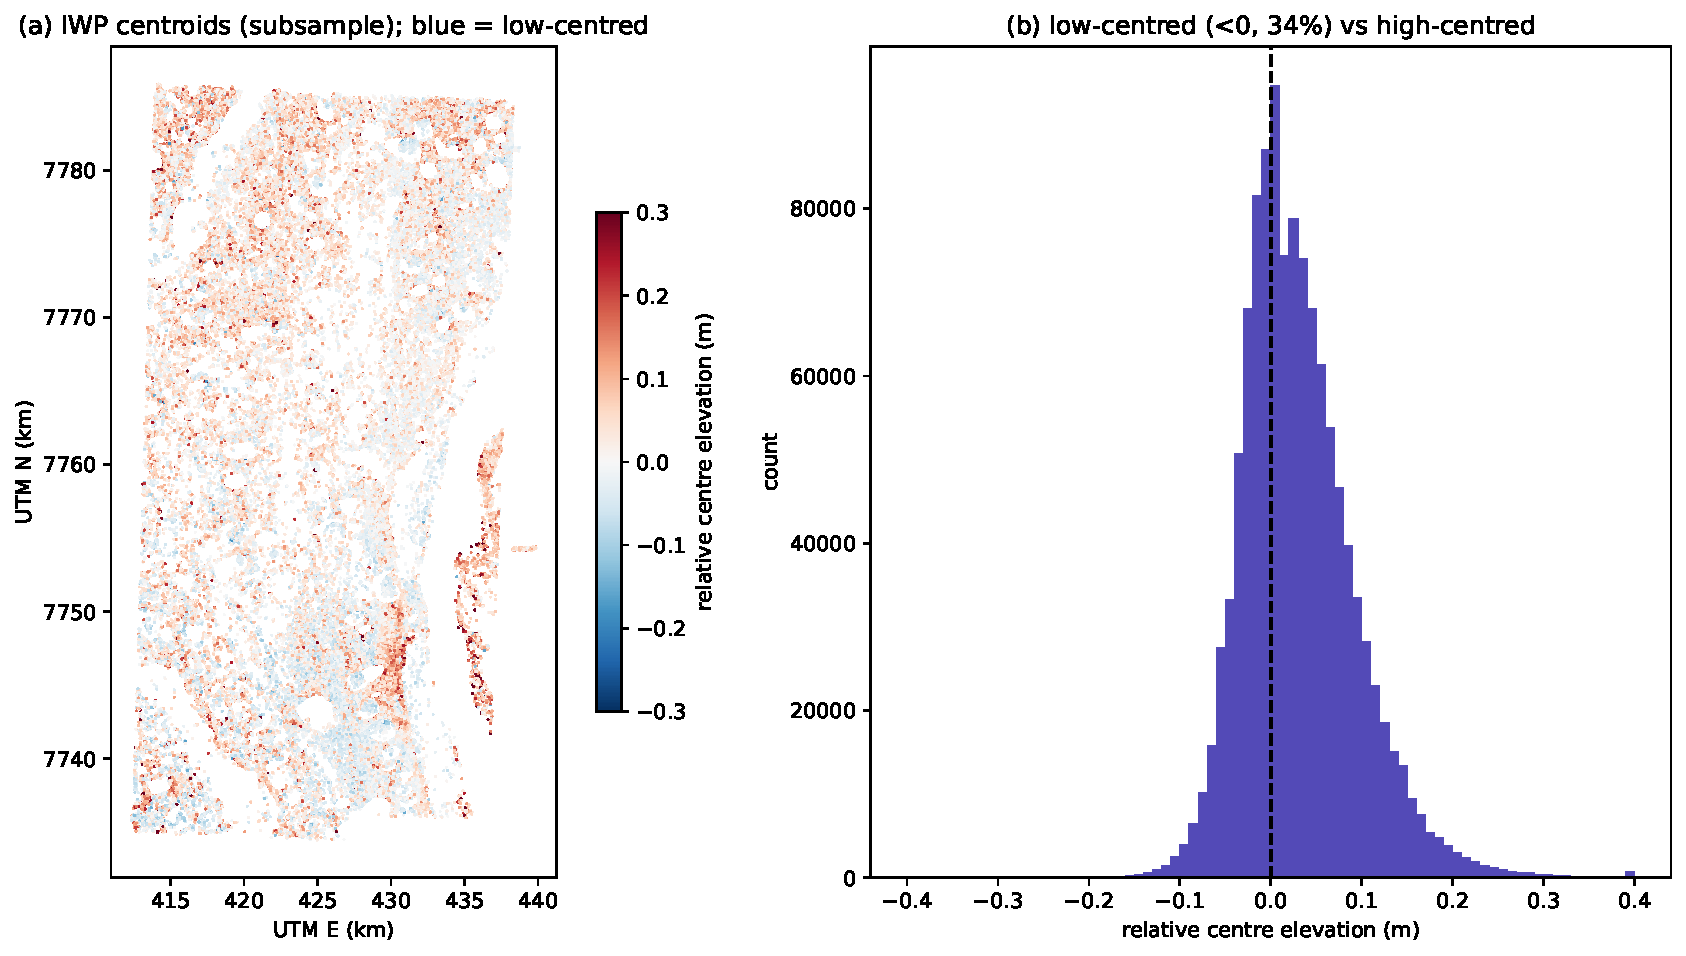
\includegraphics[width=\textwidth]{iwp_overview.pdf}
\caption{(a) Ice-wedge polygon centroids across the survey (random subsample), coloured by
relative centre elevation (blue = low-centred/intact, red = high-centred/degraded).
Polygons occur in continuous patches separated by lakes, drainage and non-polygonal ground.
(b) Distribution of relative centre elevation.}
\label{fig:overview}
\end{figure}

\section{Methods}
\paragraph{Window selection.}
The mapped polygons cover only $\sim$18\% of the survey rectangle: they form continuous,
space-filling patches separated by lakes, river corridors and non-polygonal terrain. These
gaps impose large-scale density fluctuations that would dominate the structure factor at low
wavenumber. We therefore restrict analysis to gap-free, internally homogeneous sub-windows,
selecting 1.5\,km windows by the coefficient of variation (CV) of polygon counts in 200\,m
cells (low CV = uniform coverage); we report results across the most uniform windows and, for
the degradation analysis, across 90 non-overlapping windows.

\paragraph{Point-pattern statistics.}
Within each window we compute the isotropic pair correlation $g(r)$, the radially averaged
structure factor
$S(\mathbf k)=N^{-1}\big|\sum_j e^{-i\mathbf k\cdot\mathbf r_j}\big|^2$ evaluated at the
allowed wavevectors of the window (which suppresses the window-shape artefact), and the number
variance $\sigma^2(R)$ in disks of radius $R$. Hyperuniformity requires
$S(k\!\to\!0)\!\to\!0$ and $\sigma^2(R)$ growing more slowly than $R^2$ (ideally as $R^1$ in
two dimensions) \citep{torquato2003,torquato2018}.

\paragraph{Null models.}
We compare the observed statistics against four nulls at matched density: (i) complete
spatial randomness (CSR, Poisson); (ii) an \emph{inhomogeneous}-Poisson null generated by
kernel-resampling the observed positions, which reproduces the window's large-scale density
variation but no short-range order --- a conservative control for heterogeneity; (iii) the
centroids of a \emph{Poisson--Voronoi} tessellation \citep{okabe2000}, i.e.\ a random
space-filling tessellation; and (iv) a hexagonal lattice (the ordered ceiling). The
Poisson--Voronoi comparison is the key test of whether the ice-wedge network is more ordered
than a random tessellation.

\paragraph{Degradation contrast.}
Because the intrinsic intermediate-range order ($S_{\min}$) is robust to large-scale
heterogeneity whereas the pair-correlation peak height and the number-variance exponent are
not (they correlate strongly with the density CV), we use $S_{\min}$ to compare intact and
degraded terrain, matching low-centred and high-centred windows for CV.

\section{Results}

\subsection{Local order and a characteristic spacing}
Polygon centres show clear local order (Fig.~\ref{fig:core}a): the pair correlation has a
hard core ($g\!=\!0$ below $\sim$8\,m), a sharp first peak at $\sim$15--17\,m --- the
characteristic polygon spacing --- and damped oscillations decaying to unity. This is the
signature of a dense, exclusion-dominated liquid-like arrangement.

\begin{figure}[t]
\centering

\includegraphics[width=\textwidth]{iwp_core.pdf}
\caption{Order of ice-wedge polygon centres in a representative uniform window
($N\!=\!7843$). (a) Pair correlation: hard-core exclusion and a characteristic spacing
$\sim$17\,m. (b) Structure factor: the observed $S(k)$ (purple) dips to $\approx$0.09 ---
far below the inhomogeneous-Poisson (orange) and CSR (grey) nulls, and below the
Poisson--Voronoi null (teal) --- so the network is more ordered than a random tessellation;
$S(k)$ rises again as $k\!\to\!0$. (c) Number variance grows as $R^{2.7}$, faster than the
hyperuniform $R^{1}$ (dotted) and even than Poisson $R^{2}$ at large $R$: long-range order
is not hyperuniform.}
\label{fig:core}
\end{figure}

\subsection{Intermediate-range suppression is genuine and exceeds a random tessellation}
The structure factor (Fig.~\ref{fig:core}b) shows a deep suppression, with a minimum
$S_{\min}\!\approx\!0.09$--$0.10$ at $k\!\approx\!0.16\,\mathrm{m}^{-1}$ (a scale of
$\sim$40\,m, about $2.5\times$ the spacing) in the most uniform windows. Two controls
establish that this is real order rather than an artefact of the window's density structure.
First, $S_{\min}$ lies far below the inhomogeneous-Poisson null (which is $\approx\!1$ at the
dip) in every window analysed: the suppression is not produced by the large-scale density
variation. Second, in the most uniform windows $S_{\min}$ lies below the Poisson--Voronoi
null ($\approx$0.10 versus $\approx$0.20): \emph{the ice-wedge crack network is more ordered
than a random space-filling tessellation of the same density}. The suppression is markedly
stronger than that reported for some other geological spacing patterns (Sec.~5).

\subsection{Long-range order is not hyperuniform}
Despite the deep intermediate-range dip, the pattern is not hyperuniform at long range. The
structure factor turns upward as $k\!\to\!0$ rather than vanishing, and the number variance
grows as $\sigma^2(R)\!\propto\!R^{2.7}$ (Fig.~\ref{fig:core}c) --- faster than the
hyperuniform $R^{1}$ and, at large $R$, faster even than the Poisson $R^{2}$, indicating
super-Poissonian density fluctuations at the largest scales. These fluctuations reflect real
geomorphic heterogeneity: polygon size and areal coverage vary across the landscape. Crucially,
the suppression deepens systematically in more uniform windows, which shows that the long-range
floor is set by heterogeneity (gaps, size variation), not by an intrinsic limit to the order.
A clean test of hyperuniformity would require a region of genuinely uniform polygon size, which
this mature, partly degraded landscape does not provide.

\subsection{The order survives thermokarst degradation}
Comparing intact (low-centred) and degraded (high-centred) terrain matched for density
uniformity (Fig.~\ref{fig:degrad}), both show the same hard-core spacing and a clear
intermediate-range structure-factor dip; the difference in $S_{\min}$ is weak and not
significant (medians 0.29 versus 0.22, with strongly overlapping distributions). The order is
therefore not destroyed by thermokarst: as polygons evolve from low- to high-centred, the
microtopographic relief inverts but the planimetric ice-wedge network --- and hence the
spacing order of the centres --- persists, consistent with the troughs deepening rather than
disappearing during degradation.

\begin{figure}[t]
\centering
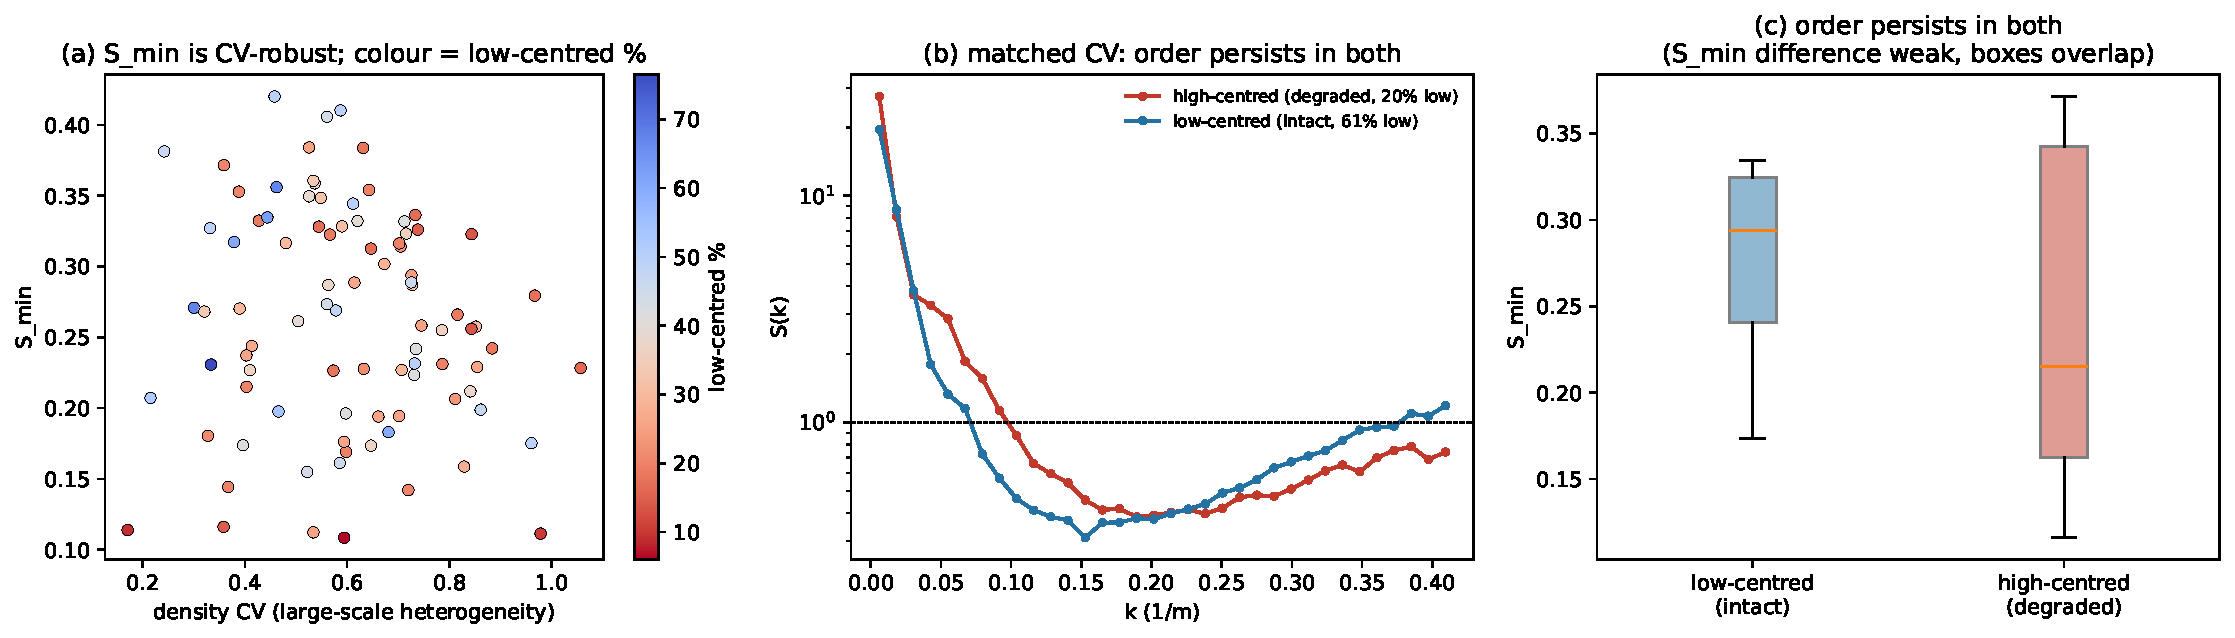
\includegraphics[width=\textwidth]{iwp_degradation.pdf}
\caption{Degradation contrast. (a) $S_{\min}$ versus the density CV across 90 windows,
coloured by low-centred fraction: $S_{\min}$ is insensitive to CV (a clean intrinsic-order
metric) and shows no strong dependence on degradation state. (b) Structure factor for an
intact (low-centred) and a degraded (high-centred) window matched in CV: both dip clearly ---
the order persists. (c) $S_{\min}$ for intact versus degraded windows in a matched-CV band:
the distributions overlap, so degradation does not destroy the intermediate-range order.}
\label{fig:degrad}
\end{figure}

\section{Discussion}

\paragraph{A fracture network more ordered than random.}
The central result is that ice-wedge polygon centres are more ordered than a Poisson--Voronoi
tessellation. This is the meaningful comparison: exceeding complete spatial randomness would be
unremarkable, because the centroids of \emph{any} space-filling tessellation avoid one another and
so appear sub-Poissonian; a random tessellation (Poisson--Voronoi) already carries that built-in
short-range order, so beating it requires the crack network itself to be regularised. Thermal-contraction
cracking is a sequential, stress-relaxing process: each new crack preferentially bisects the
largest uncracked domains and tends to meet existing cracks orthogonally, producing cells more
uniform in size than those of a random tessellation \citep{lachenbruch1962,plugwerner2002}. The
hard core in $g(r)$ is the geometric expression of this mechanism --- a thermal stress-relief halo:
once a primary contraction crack forms it relaxes the tensile stress in its surroundings, so an
adjacent parallel crack cannot nucleate within a characteristic distance \citep{lachenbruch1962}.
The deep, genuine $S(k)$ suppression ($S_{\min}\!\approx\!0.1$) is the quantitative signature of that
regularisation. We read this as a network that is geometrically optimised for strain relief, while
noting that the static spatial statistics measured here constrain the \emph{outcome} of that process,
not its dynamics directly.

\paragraph{Hyperuniform tendency, heterogeneity-limited.}
The pattern has a strong hyperuniform \emph{tendency} at intermediate scales but does not reach
confirmed long-range hyperuniformity: $S(k\!\to\!0)$ stays finite and the number variance is
super-linear, because landscape-scale variation in polygon size and coverage injects
long-wavelength density fluctuations. That the suppression deepens as windows become more uniform
identifies this as an extrinsic, heterogeneity-imposed floor rather than an intrinsic property of
the cracking process. Rather than a mere shortfall from a mathematical ideal, this long-range
heterogeneity is a geomorphic fingerprint: the wavenumber at which $S(k)$ turns up from its minimum
sets a length scale for the homogeneous polygonal patches, which on the Arctic Coastal Plain are
bounded by drained thaw-lake basins, drainage networks and gradients in ground-ice content. The
local-versus-long-range distinction --- robust local and
intermediate-range order, long-range order limited by real heterogeneity --- recurs across natural
two-dimensional spacing patterns and should be kept explicit when hyperuniformity is claimed for
field data.

\paragraph{Comparison with other geological spacing patterns.}
Among geological map patterns analysed with the same tools, ice-wedge polygons are the most
strongly suppressed at intermediate range. Salt structures, spaced by a buoyancy
(Rayleigh--Taylor) instability, form an isotropic hard-core, liquid-like regular pattern whose
intermediate-range suppression is shallower ($S_{\min}\!\approx\!0.4$;
\citealp{chen2026salt}); drumlins, shaped by directional subglacial shear, are anisotropic and
only steric-regular across flow \citep{chen2026drumlin}. Ice-wedge polygons, an isotropic
fracture tessellation with no imposed flow direction and no intrinsic basin-scale density
gradient, achieve the deepest suppression ($S_{\min}\!\approx\!0.1$). None of these field
patterns, however, reaches \emph{confirmed} long-range hyperuniformity: in every case real
geomorphic heterogeneity sets the long-wavelength floor.

\section{Conclusions}
\begin{itemize}\setlength\itemsep{1pt}
\item Ice-wedge polygon centres show hard-core exclusion and a characteristic spacing of
$\sim$15\,m, with a deep, genuine structure-factor suppression ($S_{\min}\!\approx\!0.1$) at
intermediate wavenumber.
\item In uniform windows the suppression lies below the Poisson--Voronoi null: the ice-wedge
crack network is \emph{more ordered than a random space-filling tessellation}.
\item Long-range hyperuniformity is not confirmed --- $S(k\!\to\!0)$ is finite and
$\sigma^2(R)\!\propto\!R^{2.7}$ --- because landscape heterogeneity dominates the largest scales;
the suppression deepens in more uniform windows, marking a heterogeneity-limited floor.
\item The intermediate-range order persists through the low-to-high-centred thermokarst
transition: degradation inverts the relief but preserves the planimetric network order.
\end{itemize}

\section*{Data availability}
The ice-wedge polygon inventory is from \citet{aboltyoung2020}, with data archived at PANGAEA
\citep{aboltyoung_pangaea} under CC-BY-4.0. All analysis code and derived per-window statistics
are openly available at \url{https://github.com/Ruqing1963/ice-wedge-polygon-order}. Analysis
used only open scientific Python (NumPy, SciPy, Matplotlib).

\begin{thebibliography}{99}
\small
\bibitem[Abolt \& Young(2020)]{aboltyoung2020} Abolt, C.J., Young, M.H., 2020. High-resolution
mapping of spatial heterogeneity in ice wedge polygon geomorphology near Prudhoe Bay, Alaska.
\textit{Scientific Data} 7, 87.
\bibitem[Abolt \& Young(2019)]{aboltyoung_pangaea} Abolt, C.J., Young, M.H., 2019. High-resolution
maps of ice wedge polygon occurrence and geomorphology [dataset]. PANGAEA,
doi:10.1594/PANGAEA.910178.
\bibitem[Chen(2026a)]{chen2026salt} Chen, R., 2026. Regular spacing of salt structures as a
Rayleigh--Taylor signature. Zenodo, doi:10.5281/zenodo.20834957.
\bibitem[Chen(2026b)]{chen2026drumlin} Chen, R., 2026. Anisotropic spacing of drumlins: transverse
quasi-regularity at the bedform scale versus along-flow clustering in the BRITICE record. Zenodo,
doi:10.5281/zenodo.20835748.
\bibitem[Kessler \& Werner(2003)]{kesslerwerner2003} Kessler, M.A., Werner, B.T., 2003.
Self-organization of sorted patterned ground. \textit{Science} 299, 380--383.
\bibitem[Lachenbruch(1962)]{lachenbruch1962} Lachenbruch, A.H., 1962. Mechanics of thermal
contraction cracks and ice-wedge polygons in permafrost. \textit{Geological Society of America
Special Paper} 70.
\bibitem[Okabe et al.(2000)]{okabe2000} Okabe, A., Boots, B., Sugihara, K., Chiu, S.N., 2000.
\textit{Spatial Tessellations: Concepts and Applications of Voronoi Diagrams.} Wiley.
\bibitem[Plug \& Werner(2002)]{plugwerner2002} Plug, L.J., Werner, B.T., 2002. Nonlinear dynamics
of ice-wedge networks and resulting sensitivity to severe cooling events. \textit{Nature} 417,
929--933.
\bibitem[Torquato \& Stillinger(2003)]{torquato2003} Torquato, S., Stillinger, F.H., 2003. Local
density fluctuations, hyperuniformity, and order metrics. \textit{Physical Review E} 68, 041113.
\bibitem[Torquato(2018)]{torquato2018} Torquato, S., 2018. Hyperuniform states of matter.
\textit{Physics Reports} 745, 1--95.
\end{thebibliography}

\end{document}
